\section{Cross Validation Methods}
Çapraz doğrulama, bir modelin performansını değerlendirmek için veri setini farklı parçalara böler ve her bir parça üzerinde modelin performansını değerlendirir. Bu yöntem, modelin gerçek dünya verilerine nasıl genelleme yapabileceğini daha güvenilir bir şekilde belirlemek için kullanılır. Çapraz doğrulama, aşırı uyum (overfitting) problemini önlemeye yardımcı olur ve modelin gerçek performansını daha doğru bir şekilde yansıtır.

\begin{enumerate}
    \item KFold
    \item Stratified KFold
    \item Repeated KFold
    \item Repeated Stratified KFold
    \item Leave One-Out
    \item Leave P-Out
    \item Time Series Split
\end{enumerate}

\subsection{KFold}
Veriyi rastgele parçalara böler ve modeli eğitmek ve test etmek için bu parçaları kullanır. Veri setini daha iyi kullanarak eğitim yapılmasını sağlar. Yavaş olabilir.

\subsubsection{Çalışma Adımları}
\begin{enumerate}
    \item Veri kümesi K parçaya bölünür.
    \item K parçanın her biri sırasıyla test seti olarak kullanır. Diğer k-1 parçayı eğitim seti olarak kullanır. 
    \item Model K kez eğitilir ve test edilir.
    \item Her bir eğitim-test işlemi sonucunda elde edilen performans ölçümleri ortalanır.
\end{enumerate}

\newpage

\begin{figure}[h]
    \centering
    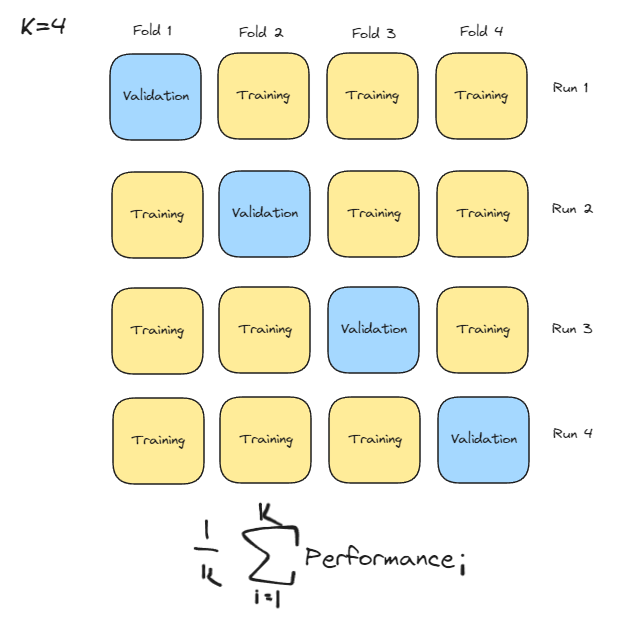
\includegraphics[width=1\textwidth]{images/kfold_structure.png}
    \caption{KFold.}
    \label{fig:enter-label}
\end{figure}

\begin{lstlisting}[language=Python, caption=Scikit-learn'de KFold örneği.]
from sklearn.model_selection import KFold
from sklearn.linear_model import LinearRegression
import numpy as np

X = np.array([[1, 2], [3, 4], [5, 6], [7, 8]])
y = np.array([11, 12, 13, 14])

kf = KFold(n_splits=2)

for train_index, test_index in kf.split(X):
    X_train, X_test = X[train_index], X[test_index]
    y_train, y_test = y[train_index], y[test_index]
    
    model = LinearRegression()
    model.fit(X_train, y_train)
    
    score = model.score(X_test, y_test)
    print("Test seti skoru:", score)
\end{lstlisting}

\subsection{Stratified KFold}
KFold gibi çalışır fakat her katmanın sınıf dağılımını korumak için sınıfları dengeli bir şekilde böler. Sınıf dengesizliği durumunda daha güvenilir sonuçlar sağlar. Sınıf dağılımını koruyarak her katmanda her sınıfın temsil edilmesini sağlar. Stratifikasyon her zaman mümkün olmayabilir.

\subsubsection{Çalışma Adımları}
\begin{enumerate}
    \item Veri kümesi k parçaya bölünür.
    \item Her bir parçanın sınıf dağılımını KFold gibi böler.
    \item Her parça, orijinal veri setindeki sınıf oranlarını yansıtacak şekilde oluşturulur.
    \item Model K kez eğitilir ve test edilir, her seferinde farklı bir parça test seti olarak seçilir.
\end{enumerate}

\begin{figure}[h]
    \centering
    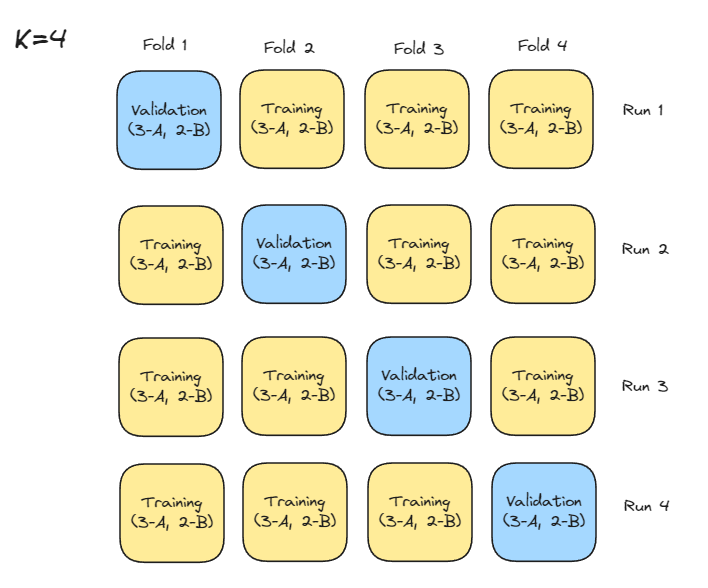
\includegraphics[width=0.8\textwidth]{images/stratified_kfold_structure.png}
    \caption{Stratified KFold.}
    \label{fig:enter-label}
\end{figure}

\begin{lstlisting}[language=Python, caption=Scikit-learn'de Stratified KFold örneği.]
from sklearn.model_selection import StratifiedKFold
from sklearn.datasets import make_classification
from sklearn.linear_model import LogisticRegression

X, y = make_classification(n_samples=100, n_features=4, n_informative=2, n_redundant=0, random_state=42, n_classes=2)

skf = StratifiedKFold(n_splits=3)

for train_index, test_index in skf.split(X, y):
    X_train, X_test = X[train_index], X[test_index]
    y_train, y_test = y[train_index], y[test_index]
    
    model = LogisticRegression()
    model.fit(X_train, y_train)
    
    score = model.score(X_test, y_test)
    print("Test seti skoru:", score)
\end{lstlisting}

\subsection{Repeated KFold}
Veri kümesini KFold yöntemiyle bölmenin tekrarlanabilir bir versiyonudur. Bir KFold çapraz doğrulama işlemini belirli bir sayıda tekrarlayarak daha güvenilir bir performans tahmini elde etmeyi amaçlar. Veri kümesi dengeli ise gereksiz olabilir.

\subsubsection{Çalışma Adımları}
\begin{enumerate}
    \item Veri kümesi k parçaya bölünür.
    \item Bu K parçayı kullanarak model eğitilir ve test edilir.
    \item İşlem belirli bir sayıda tekrarlanır.
    \item Her tekrarda farklı rastgele parçalar seçilir.
\end{enumerate}

\begin{lstlisting}[language=Python, caption=Scikit-learn'de Repeated KFold örneği.]
from sklearn.model_selection import RepeatedKFold
from sklearn.datasets import make_regression
from sklearn.linear_model import LinearRegression

X, y = make_regression(n_samples=100, n_features=2, noise=0.1, random_state=42)

rkf = RepeatedKFold(n_splits=3, n_repeats=2)

for train_index, test_index in rkf.split(X):
    X_train, X_test = X[train_index], X[test_index]
    y_train, y_test = y[train_index], y[test_index]
    
    model = LinearRegression()
    model.fit(X_train, y_train)
    
    score = model.score(X_test, y_test)
    print("Test seti skoru:", score)
\end{lstlisting}


\subsection{Repeated Stratified KFold}
StratifiedKFold'un tekrarlanabilir bir versiyonudur. Sınıflandırma problemlerinde kullanılan ve sınıf dengesini koruyarak veri setini tekrarlayan bir çapraz doğrulama tekniğidir.

\subsubsection{Çalışma Adımları}
\begin{enumerate}
    \item Veri kümesi StratifiedKFold gibi sınıf dengesini koruyarak K parçaya bölünür.
    \item Bu K parçayı kullanarak modeli eğitir ve test eder.
    \item İşlem belirli bir sayıda tekrarlanır.
    \item Her tekrarda farklı rastgele parçalar seçilir.
\end{enumerate}

\begin{lstlisting}[language=Python, caption=Scikit-learn'de Repeated Stratified KFold örneği.]
from sklearn.model_selection import RepeatedStratifiedKFold
from sklearn.datasets import make_classification
from sklearn.ensemble import RandomForestClassifier

X, y = make_classification(n_samples=100, n_features=4, n_informative=2, n_redundant=0, random_state=42, n_classes=2)

rskf = RepeatedStratifiedKFold(n_splits=3, n_repeats=2, random_state=42)

for train_index, test_index in rskf.split(X, y):
    X_train, X_test = X[train_index], X[test_index]
    y_train, y_test = y[train_index], y[test_index]
    
    model = RandomForestClassifier()
    model.fit(X_train, y_train)
    
    score = model.score(X_test, y_test)
    print("Test seti skoru:", score)
\end{lstlisting}


\subsection{Leave One-Out}
Veri setinin her bir örneğini sadece bir kez test seti olarak kullanarak gerçekleştirilir. Her bir veri noktası sırasıyla test edilirken geri kalanı eğitim seti olarak kullanılır.

\subsubsection{Çalışma Adımları}
\begin{enumerate}
    \item Veri kümesi içindeki her bir örnek sırayla test seti olarak seçilir.
    \item Seçilen örnek dışındaki tüm veri eğitim seti olarak kullanılır.
    \item Model, seçilen örneği test etmek ve performansını ölçmek için eğitilir.
    \item Bu işlem tüm veri noktaları için tekrarlanır.
\end{enumerate}

\begin{figure}[h]
    \centering
    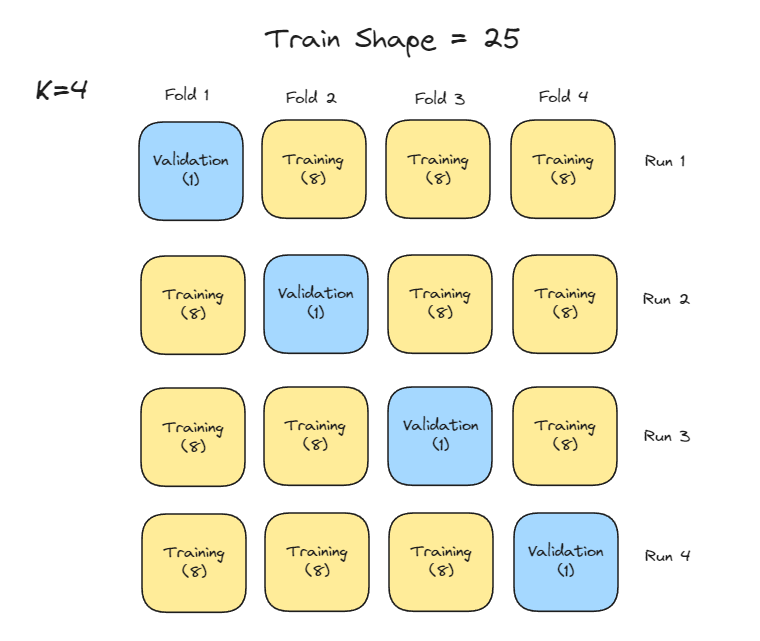
\includegraphics[width=1\textwidth]{images/leave_one_out_structure.png}
    \caption{Leave One-Out.}
    \label{fig:enter-label}
\end{figure}

\begin{lstlisting}[language=Python, caption=Scikit-learn'de Leave One-Out örneği.]
from sklearn.model_selection import LeaveOneOut
from sklearn.datasets import load_iris
from sklearn.neighbors import KNeighborsClassifier

iris = load_iris()
X = iris.data
y = iris.target

loo = LeaveOneOut()

accuracies = []
for train_index, test_index in loo.split(X):
    X_train, X_test = X[train_index], X[test_index]
    y_train, y_test = y[train_index], y[test_index]
    
    model = KNeighborsClassifier()
    model.fit(X_train, y_train)
    
    accuracy = model.score(X_test, y_test)
    accuracies.append(accuracy)

mean_accuracy = sum(accuracies) / len(accuracies)
print("Ortalama dogruluk:", mean_accuracy)
\end{lstlisting}

\subsection{Leave P-Out}
Her bir iterasyonda P öğeyi test seti olarak kullanarak gerçekleştirilir. LOO (Leave One-Out) ve KFold'un genelleştirilmiş bir versiyonudur. LOO, P=1 olduğunda Leave P-Out'a eşittir.

\subsubsection{Çalışma Adımları}
\begin{enumerate}
    \item Veri kümesinde P öğeyi test seti olarak bırakır, geri kalanını eğitim seti olarak kullanır.
    \item Model, test setindeki öğeleri tahmin etmek ve performansını ölçmek için eğitilir.
    \item Bu işlem veri kümesindeki her bir P öğesi için tekrarlanır.
\end{enumerate}

\newpage

\begin{figure}[h]
    \centering
    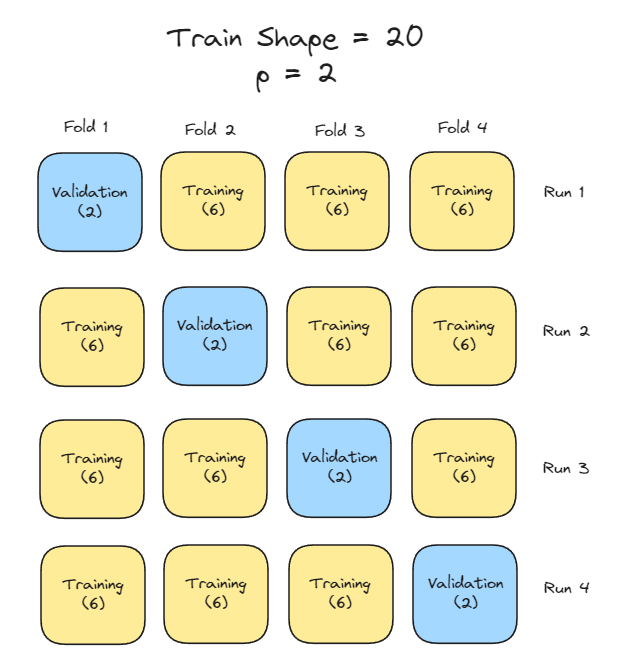
\includegraphics[width=1\textwidth]{images/leave_p_out_structure.png}
    \caption{Leave P-Out.}
    \label{fig:enter-label}
\end{figure}

\begin{lstlisting}[language=Python, caption=Scikit-learn'de Leave P-Out örneği.]
from sklearn.model_selection import LeavePOut
from sklearn.datasets import load_iris
from sklearn.neighbors import KNeighborsClassifier

iris = load_iris()
X = iris.data
y = iris.target

lpout = LeavePOut(p=2)

accuracies = []
for train_index, test_index in lpout.split(X):
    X_train, X_test = X[train_index], X[test_index]
    y_train, y_test = y[train_index], y[test_index]
    
    model = KNeighborsClassifier()
    model.fit(X_train, y_train)
    
    accuracy = model.score(X_test, y_test)
    accuracies.append(accuracy)

mean_accuracy = sum(accuracies) / len(accuracies)
print("Ortalama dogruluk:", mean_accuracy)
\end{lstlisting}


\subsection{Time Series Split}
Zaman serisi veri setlerinde kullanılan çapraz doğrulama yöntemlerinden biridir. Zaman serileri için veriyi bölme ve çapraz doğrulama yapma işlemidir.

\subsubsection{Çalışma Adımları}
\begin{enumerate}
    \item Veri, kronolojik sıraya göre (zaman bileşeni) parçalara bölünür.
    \item Her bir bölüm, eğitim ve test setleri olarak kullanılır.
    \item Örneğin, ilk k-1 bölüm eğitim seti, k. bölüm test seti olarak kullanılabilir.
    \item Bu işlem bir döngü içinde tekrarlanarak farklı eğitim ve test setleri elde edilir.
\end{enumerate}

\newpage

\begin{figure}[h]
    \centering
    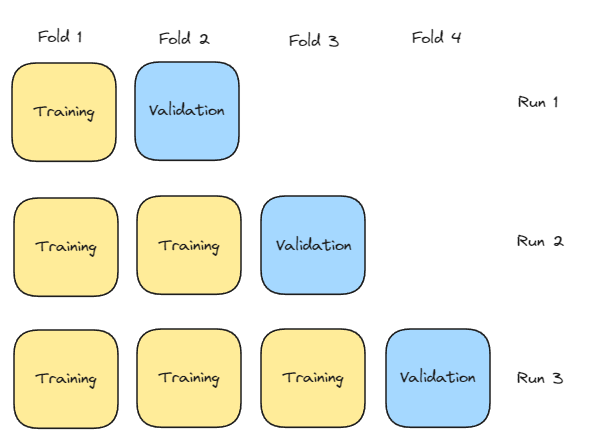
\includegraphics[width=1\textwidth]{images/time_series_split_structure.png}
    \caption{Time Series Split.}
    \label{fig:enter-label}
\end{figure}

\begin{lstlisting}[language=Python, caption=Scikit-learn'de Time Series Split örneği.]
from sklearn.model_selection import TimeSeriesSplit
import numpy as np

time_series = np.array([1, 2, 3, 4, 5, 6, 7, 8, 9, 10])

tscv = TimeSeriesSplit(n_splits=3)

for train_index, test_index in tscv.split(time_series):
    train_data, test_data = time_series[train_index], time_series[test_index]
    
    print("Egitim seti:", train_data)
    print("Test seti:", test_data)
    print("------")
\end{lstlisting}

\newpage